\documentclass[prx,12pt]{revtex4-2}
\usepackage{amsmath}
\usepackage{amssymb}
\usepackage{graphicx}
\usepackage{color}
\usepackage{enumerate}
\usepackage{framed}
\usepackage[pdfborder={0 0 0},colorlinks=true,linkcolor=blue,urlcolor=blue]{hyperref}

\def\ket#1{\left|#1\right\rangle}
\def\bra#1{\left\langle#1\right|}
\def\braket#1{\left\langle#1\right\rangle}

\usepackage{fancyhdr}
\fancyhf{}
\lhead{\tiny Y.~D.~Chong}
\rhead{\scriptsize Ch.~1: Scattering Theory $|$ Graduate Quantum Mechanics}
\lfoot{}
\rfoot{\thepage}
\pagestyle{fancy}

\renewcommand{\theequation}{1.\arabic{equation}}

\setlength{\parindent}{14pt}

\renewcommand{\baselinestretch}{1.0}
\setlength{\parskip}{0.04in}

\def\thesection{1.\arabic{section}}
\def\thesubsection{\thesection.\arabic{subsection}}

\makeatletter
\renewcommand{\p@subsection}{}
\renewcommand{\p@subsubsection}{}
\makeatother

\begin{document}

\begin{center}
{\Large \textbf{Chapter 1: Scattering Theory}}
\end{center}

%% \section{Scattering Processes in Quantum Mechanics}

\section{Scattering experiments on quantum particles}
\label{sec:scatintro}

Quantum particles exhibit a feature known as \textbf{wave-particle
  duality}, which can be summarized in the \textbf{quantum double-slit
  thought experiment}.  As illustrated below, a source emits electrons
of energy $E$ toward a screen with a pair of slits.  A movable
detector, placed on the far side, measures the arrival rates at
different positions.

\begin{figure}[h]
  \centering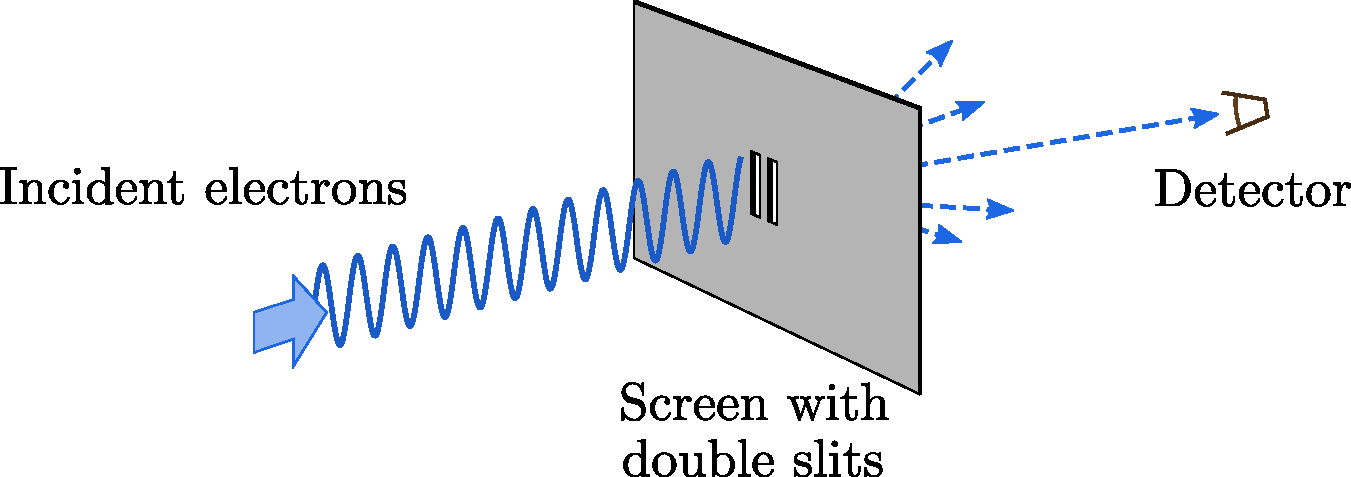
\includegraphics[width=0.52\textwidth]{doubleslit}
\end{figure}

The experiment reveals the following: (i) the electrons arrive in
discrete units, like classical particles; (ii) the
\textit{statistical} distribution of electron arrivals forms an
interference pattern, like a diffracted wave.  In the non-relativistic
limit, the inferred wavelength $\lambda$ is related to the electron
energy $E$ by
\begin{equation}
  \lambda = \frac{2\pi}{k}, \;\;\; E = \frac{\hbar^2k^2}{2m},
\end{equation}
where $\hbar = h/2\pi$ is Dirac's constant, and $m$ is the electron
mass.  (Thus, if $E$ is known, we can deduce the spacing of the slits
from the diffraction pattern.)

%% Wave-particle duality arises from quantum theory's distinction between
%% a particle's state and the outcomes of measurements performed on it.
%% The state is described by a wavefunction $\psi(\mathbf{r})$, which can
%% undergo diffraction like a classical wave.  On the other hand, the
%% probability of measuring a particle in a volume $dV$ around position
%% $\mathbf{r}$ is given by $|\psi(\mathbf{r})|^2 \,dV$.

In this chapter, we will study a generalization of the double-slit
experiment called a \textbf{scattering experiment}.  The idea is to
shoot quantum particles at a target, called a \textbf{scatterer}, and
measure the distribution of scattered particles.  Just as the
double-slit interference pattern can be used to deduce the slit
spacing, a scattering experiment can be used to deduce various facts
about the scatterer.  Scattering experiments constitute a large
proportion of the methods used to probe the quantum world, from
electron- and photon-based microscopy to accelerator experiments in
high-energy physics.

We will focus on the non-relativistic scattering experiment depicted
below:

\begin{figure}[h]
  \centering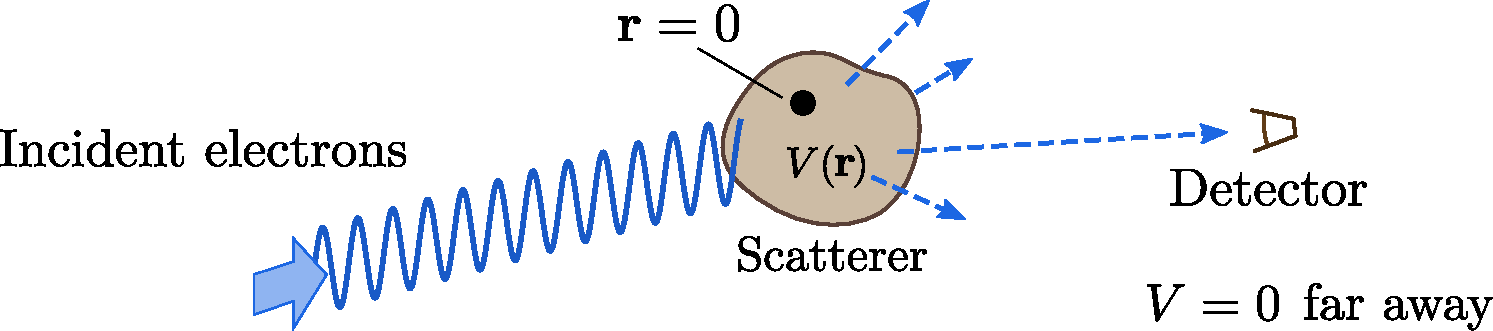
\includegraphics[width=0.58\textwidth]{scattering}
\end{figure}

\noindent
An unbounded $d$-dimensional space is described
by coordinates $\mathbf{r}$, with a scatterer near $\mathbf{r} = 0$.
An incoming quantum particle, with energy $E$, is governed by the
Hamiltonian
\begin{equation}
  \hat{H} = \hat{H}_0 + V(\hat{\mathbf{r}}),
\end{equation}
where
\begin{equation}
  \hat{H}_0 = \frac{\hat{\mathbf{p}}^2}{2m}
\end{equation}
describes the particle's kinetic energy, $m$ is the particle's mass,
$\hat{\mathbf{r}}$ and $\hat{\mathbf{p}}$ are the position and
momentum operators, and $V$ is a \textbf{scattering potential}
describing how the scatterer acts upon the particle.  We assume this
potential vanishes far from the scatterer:
\begin{equation}
  V(\mathbf{r}) \; \overset{|\mathbf{r}| \rightarrow \infty}{\longrightarrow}\; 0.
\end{equation}

How is the particle scattered by the potential?  In order to study
this, we formulate the above description as the following mathematical
problem:
\begin{enumerate}
\item 
A particle state $|\psi\rangle$ obeys the time-independent
Schr\"odinger equation
\begin{equation}
  \hat{H} |\psi\rangle = E |\psi\rangle,
  \label{scatter1}
\end{equation}
where $E$ is the incoming particle energy.

\item
The state $|\psi\rangle$ can be decomposed into two pieces,
\begin{equation}
  |\psi\rangle \,=\, |\psi_i\rangle \,+\, |\psi_s\rangle,
  \label{scatter2}
\end{equation}
where $|\psi_i\rangle$ is called the \textbf{incident state} and
$|\psi_s\rangle$ is called the \textbf{scattered state}.

\item
The incident state is described by a plane wave, which is a
simultaneous eigenstate of $\hat{H}_0$ (with energy $E$) and
$\hat{\mathbf{p}}$ (with momentum $\mathbf{p}_i$):
\begin{equation}
  \begin{cases}
  \hat{H}_0 |\psi_i\rangle &= \, E |\psi_i\rangle, \\
  \;\;\hat{\mathbf{p}} |\psi_i\rangle &= \, \mathbf{p}_i |\psi_i\rangle,
  \end{cases}
  \quad \mathrm{where} \;\;\; E = \frac{|\mathbf{p}_i|^2}{2m}.
  \label{scatter3}
\end{equation}

\item
The scattered state is an ``outgoing'' state.  What this means will be
explained later.
\end{enumerate}
We can interpret the above statements as follows.  Statement 1 says the
scattering is elastic: the scatterer is described by a potential
$V(\mathbf{r})$, so its interaction with the particle is conservative
and $E$ is fixed.  Statement 2 says that the wavefunction
$\psi(\mathbf{r}) = \langle \mathbf{r} |\psi\rangle$ is a
superposition of an incoming wave and a scattered wave.  Statement 3
defines the incoming wave as a plane wave with wavelength determined
by $E$.  Statement 4 says the scattered wave moves outward to
infinity, away from the scatterer.

Note that Statements 1--4 do \textit{not} define an eigenproblem!
Usually, we deal with the time-independent Schr\"odinger equation by
finding eigenvalues and eigenstates.  But here we are given
$|\psi_i\rangle$, $E$, and $V(\mathbf{r})$, and want $|\psi_s\rangle$.
In particular, $E$ is an input to the calculation (a continuously
variable parameter), not an output (an eigenvalue).

\section{Recap: position and momentum states}
\label{sec:waves}

Before proceeding, let us review the properties of a quantum particle
in free space.  In a $d$-dimensional space, a coordinate vector
$\mathbf{r}$ is a real vector with $d$ components.  We suppose there
is a uncountably infinite set of position eigenstates,
$\{|\mathbf{r}\rangle\}$, where each $|\mathbf{r}\rangle$ describes a
particle with a definite position $\mathbf{r}$.  The position
eigenstates are assumed to span the state space, such that the
identity operator can be resolved as
\begin{equation}
  \hat{I} = \int d^dr \, |\mathbf{r}\rangle \langle\mathbf{r}|,
  \label{Iresol}
\end{equation}
with the integral is taken over all allowed $\mathbf{r}$ (e.g.,
$\mathbf{r} \in \mathbb{R}^d$).  It follows that
\begin{equation}
  \langle \mathbf{r} | \mathbf{r}' \rangle = \delta^d(\mathbf{r}-\mathbf{r}').
  \label{rrprime}
\end{equation}
Thus, we say that the position eigenstates are
\textbf{delta-normalized}, rather than being normalized to unity.
Here $\delta^d(\cdots)$ denotes the $d$-dimensional delta function;
e.g., in 2D,
\begin{equation*}
  \langle x,y \,|\, x',y' \rangle = \delta(x-x') \, \delta(y-y').
\end{equation*}
Moreover, the position operator $\hat{\mathbf{r}}$ is defined such
that $\hat{\mathbf{r}} |\mathbf{r}\rangle \,=\, \mathbf{r}\,
|\mathbf{r}\rangle$.

Momentum eigenstates are constructed from position eigenstates via
Fourier transforms.  First, let us suppose $\mathbf{r}$ runs over a
finite box of length $L$ on each side, with periodic boundary
conditions.  For plane waves of the form
$\exp(i\mathbf{k}\cdot\mathbf{r})$, where $\mathbf{k} = (k_1, \dots,
k_d)$ is the wave-vector, the periodic boundary conditions are
satisfied if and only if
\begin{equation}
  k_j = 2\pi m/L\;\;\mathrm{for} \;m\in\mathbb{Z}.
\end{equation}
Note that the set of allowed wave-vectors is discrete (i.e.,
countable), with a discretization of $\Delta k = 2\pi/L$ in each
direction.  Next, define
\begin{equation}
  |\mathbf{k}\rangle = \frac{1}{L^{d/2}} \, \int d^dr \; e^{i\mathbf{k}\cdot\mathbf{r}} |\mathbf{r}\rangle,
  \label{pdef}
\end{equation}
where the integral is taken over the box.  We identify
$|\mathbf{k}\rangle$ as a momentum eigenstate, i.e., a state with
definite momentum $\hbar \mathbf{k}$.  Using
Eqs.~\eqref{Iresol}--\eqref{rrprime} and Eq.~\eqref{pdef}, we can show
that
\begin{equation}
  \langle\mathbf{k}|\mathbf{k}'\rangle = \delta_{\mathbf{k},\mathbf{k}'}, \quad \langle\mathbf{r}|\mathbf{k}\rangle = \frac{1}{L^{d/2}} e^{i\mathbf{k}\cdot\mathbf{r}}, \quad I = \sum_{\mathbf{k}} |\mathbf{k}\rangle\,\langle\mathbf{k}|.
\end{equation}
In particular, note that each momentum eigenstate is normalizable to
unity.

Now let us take $L \rightarrow \infty$.  In this limit, the
wave-vector discretization $\Delta k = 2\pi / L$ goes to zero, so the
momentum eigenvalues coalesce into a continuum.  To handle this, we
redefine the momentum eigenstates as
\begin{equation}
  |\mathbf{k}\rangle^{(\textrm{new})} = \left(\frac{L}{2\pi}\right)^{d/2} |\mathbf{k}\rangle^{(\textrm{old})}.
\end{equation}
Then, by using the formula
\begin{equation}
  \int_{-\infty}^\infty dx\; \exp(ikx) \;=\; 2\pi\, \delta(k),
\end{equation}
we can show that the new momentum eigenstates are related to the
position eigenstates by
\begin{framed}
  \begin{align}
      |\mathbf{k}\rangle &= \frac{1}{(2\pi)^{d/2}} \, \int d^dr \; e^{i\mathbf{k}\cdot\mathbf{r}} |\mathbf{r}\rangle, \label{kcontdef} \\
      |\mathbf{r}\rangle &= \frac{1}{(2\pi)^{d/2}} \, \int d^dk \; e^{-i\mathbf{k}\cdot\mathbf{r}} |\mathbf{k}\rangle. \label{rcontdef}
  \end{align}
\end{framed}
\vskip -0.1in
\noindent
Position and momentum are now treated on similar footing, with the
integrals over $\mathbf{r}$ and $\mathbf{k}$ both taken over infinite
spaces.  Moreover, the momentum eigenstates now satisfy
\begin{align}
  I &= \int d^dk \;|\mathbf{k}\rangle\,\langle\mathbf{k}|, \label{Iresolk} \\
  \langle\mathbf{k}|\mathbf{k}'\rangle &= \delta^d(\mathbf{k}-\mathbf{k}'),
  \label{kkprime} \\
  \langle\mathbf{r}|\mathbf{k}\rangle &= \frac{e^{i\mathbf{k}\cdot\mathbf{r}}}{(2\pi)^{d/2}}. \label{kwavefun}
\end{align}
The first two equations are analogous to their position eigenstate
counterparts, Eq.~\eqref{Iresol} and \eqref{rrprime}.  In particular,
Eq.~\eqref{kkprime} says the new $|\mathbf{k}\rangle$'s are
delta-normalized.  The last equation, \eqref{kwavefun}, can be
interpreted as the wavefunction of the delta-normalized momentum
eigenstate.

The momentum operator $\hat{\mathbf{p}}$ is defined using the
$|\mathbf{k}\rangle$'s as the eigenbasis:
\begin{equation}
  \hat{\mathbf{p}} |\mathbf{k}\rangle \,=\, \hbar \mathbf{k}\, |\mathbf{k}\rangle.
  \label{pop}
\end{equation}
For any quantum state $|\psi\rangle$, whose wavefunction is
$\psi(\mathbf{r}) = \langle \mathbf{r}|\psi\rangle$, we can use
Eqs.~\eqref{rcontdef} and \eqref{pop} to show that the momentum
operator acts on wavefunctions in the following way:
\begin{align}
  \begin{aligned}\langle \mathbf{r}|\hat{\mathbf{p}}|\psi\rangle
    &= \frac{1}{(2\pi)^{d/2}} \, \int d^dk \; e^{i\mathbf{k}\cdot\mathbf{r}} \langle \mathbf{k} | \hat{\mathbf{p}} | \psi\rangle \\
    &= \frac{1}{(2\pi)^{d/2}} \, \int d^dk \; \hbar\mathbf{k} \, e^{i\mathbf{k}\cdot\mathbf{r}} \langle \mathbf{k} | \psi\rangle \\
    &= -i \hbar\nabla \left[\frac{1}{(2\pi)^{d/2}} \, \int d^dk \, e^{i\mathbf{k}\cdot\mathbf{r}} \langle \mathbf{k} | \psi\rangle \right] \\
    &= -i\hbar \nabla\psi(\mathbf{r}).
  \end{aligned}
\end{align}

\section{Scattering from a 1D delta function potential}
\label{sec:1dscatter}

We are now ready to solve a simple scattering problem.  Consider a 1D
space with spatial coordinate $x$, and a scattering potential
consisting of a ``spike'' at $x = 0$:
\begin{equation}
  V(x) = \frac{\hbar^2\gamma}{2m} \,\delta(x).
  \label{Vdeltaf}
\end{equation}
The form of the prefactor $\hbar^2\gamma/2m$ is chosen for later
convenience; the parameter $\gamma$, which has units of $[1/x]$,
controls the strength of the scattering potential.

\begin{figure}[h]
  \centering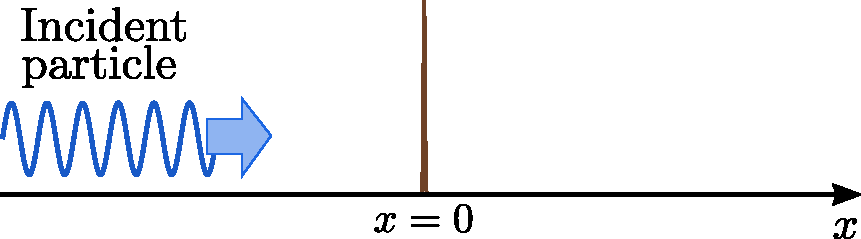
\includegraphics[width=0.45\textwidth]{scattering1d}
\end{figure}

The particle wavefunction $\psi(x)$ satisfies the 1D Schr\"odinger
wave equation
\begin{equation}
  \left[-\frac{\hbar^2}{2m} \frac{d^2}{dx^2} + V(x) \right] \psi(x)
  = E \psi(x).
  \label{1dschrod}
\end{equation}
As this is a second-order differential equation, we normally require
$\psi(x)$ to be continuous and to have well-defined first and second
derivatives.  However, the delta function potential \eqref{Vdeltaf}
relaxes these requirements in a peculiar way: at $x=0$, $\psi(x)$ must
still be continuous, but its first derivative may now be discontinuous
(and hence, its second derivative is singular).  To see this,
integrate Eq.~\eqref{1dschrod} over an infinitesimal range around $x =
0$:
\begin{align}
  \begin{aligned}\lim_{\varepsilon\rightarrow 0^+} \int_{-\varepsilon}^{+\varepsilon} dx\; \left[-\frac{\hbar^2}{2m} \frac{d^2}{dx^2} + \frac{\hbar^2\gamma}{2m} \delta(x)\right] \psi(x) &= \lim_{\varepsilon\rightarrow 0^+} \int_{-\varepsilon}^{+\varepsilon} dx\; E \psi(x) \\ = \lim_{\varepsilon\rightarrow 0^+} \left(-\frac{\hbar^2}{2m} \left[\frac{d\psi}{dx}\right]_{-\varepsilon}^{+\varepsilon} \right) + \frac{\hbar^2\gamma}{2m} \psi(0) &= 0.
  \end{aligned}
\end{align}
Therefore,
\begin{equation}
  \lim_{\varepsilon\rightarrow 0^+} \left(\; \left.\frac{d\psi}{dx}\right|_{x = +\varepsilon} - \;\; \left.\frac{d\psi}{dx}\right|_{x = -\varepsilon}\; \right) =  \gamma \,\psi(0).
  \label{delta_discontinuity}
\end{equation}

In accordance our previously-discussed formulation of the scattering
problem, and specifically Eq.~\eqref{scatter2}, the total wavefunction
is split into
\begin{equation}
  \psi(x) = \psi_i(x) + \psi_s(x).
\end{equation}
Moreover, the incident state should be a momentum eigenstate.  But we
will \textit{not} let it be delta-normalized, as momentum eigenstates
normally are (see Sec.~\ref{sec:waves}).  Instead, we write
\begin{equation}
  \psi_i(x) = \Psi_i \, e^{ik x},
  \;\;\;k = \sqrt{\frac{2mE}{\hbar^2}} > 0.
  \label{psiin1d}
\end{equation}
The complex coefficient $\Psi_i$ is called the \textbf{incident
  amplitude}.  Introducing $\Psi_i$ in this way emphasizes that the
magnitude and phase of the incident wavefunction are, in principle,
adjustable parameters in the scattering experiment.  In terms of the
usual delta-normalized momentum eigenstates,
\begin{equation}
  |\psi_i\rangle = \sqrt{2\pi}\, \Psi_i |k\rangle.
\end{equation}

With this, Eq.~\eqref{1dschrod} becomes
\begin{equation}
  \left[-\frac{\hbar^2}{2m} \frac{d^2}{dx^2} + \frac{\hbar^2\gamma}{2m}\delta(x)\right] \Big(\Psi_i \, e^{ikx} + \psi_s(x) \Big)
  = E \Big(\Psi_i \, e^{ikx} + \psi_s(x) \Big).
\end{equation}
Taking $E = \hbar^2k^2/2m$, and doing a bit of algebra, simplifies this to
\begin{equation}
  \left[ \frac{d^2}{dx^2} + k^2\right] \psi_s(x)
  = \gamma \delta(x) \Big(\Psi_i \, e^{ikx} + \psi_s(x) \Big).
  \label{deltaschrod}
\end{equation}

We can construct the solution by separately considering the regions $x
< 0$ and $x > 0$.  Within each half-space, $\delta(x)$ vanishes so
Eq.~\eqref{deltaschrod} reduces to the Helmholtz equation
\begin{equation}
  \left[\frac{d^2}{dx^2} + k^2\right] \psi_s(x) = 0.
\end{equation}
This has the general solution
\begin{equation}
  \psi_s(x) = \Psi_i \left(f_R \, e^{ik x} + f_L \, e^{-ik x}\right),
\end{equation}
which is a superposition of right-moving ($e^{ikx}$) and left-moving
($e^{-ikx}$) waves.  The complex parameters $f_1$ and $f_2$ can
have different values in the $x < 0$ and $x > 0$ regions.

We want the scattered wave to be an outgoing wave.  Thus, for $x < 0$,
$\psi_s$ is purely left-moving, so $f_R = 0$; and for $x > 0$,
$\psi_s$ is purely right-moving, so $f_L = 0$.  Therefore,
\begin{equation}
  \psi_s(x) = \Psi_i \times \begin{cases}f_- \,e^{-ikx}, & x < 0 \\ f_+ \,e^{ikx}, & x > 0.\end{cases}
\end{equation}
The complex numbers $f_-$ and $f_+$ are called \textbf{scattering
  amplitudes}.  They parameterize the magnitude and phase of the
scattered wavefunction moving outward from the scatterer.

Recall from the discussion at the beginning of this section that
$\psi(x)$ must be continuous at $x = 0$.  This implies that
$\psi_s(x)$ is also continuous, and therefore that
\begin{equation}
  f_- = f_+ \;\;\;\Rightarrow \;\;\;
  \psi_s(x) = \Psi_i \,f_\pm\, e^{ik|x|}.
  \label{psis1d}
\end{equation}
Plugging Eqs.~\eqref{psiin1d} and \eqref{psis1d} into
Eq.~\eqref{delta_discontinuity} yields
\begin{equation}
  f_\pm = -\frac{\gamma}{\gamma - 2ik}.
\end{equation}

For now, let us focus on the magnitude of the scattering amplitude (in
the next chapter, we will see that the phase also contains useful
information).  The quantity $|f_\pm|^2$ describes the overall strength
of the scattering process:
\begin{equation}
  |f_\pm|^2 = \left[1 + \frac{8mE}{(\hbar\gamma)^2}\right]^{-1}.
\end{equation}
Its dependence on $E$ is plotted below:

\begin{figure}[h]
  \centering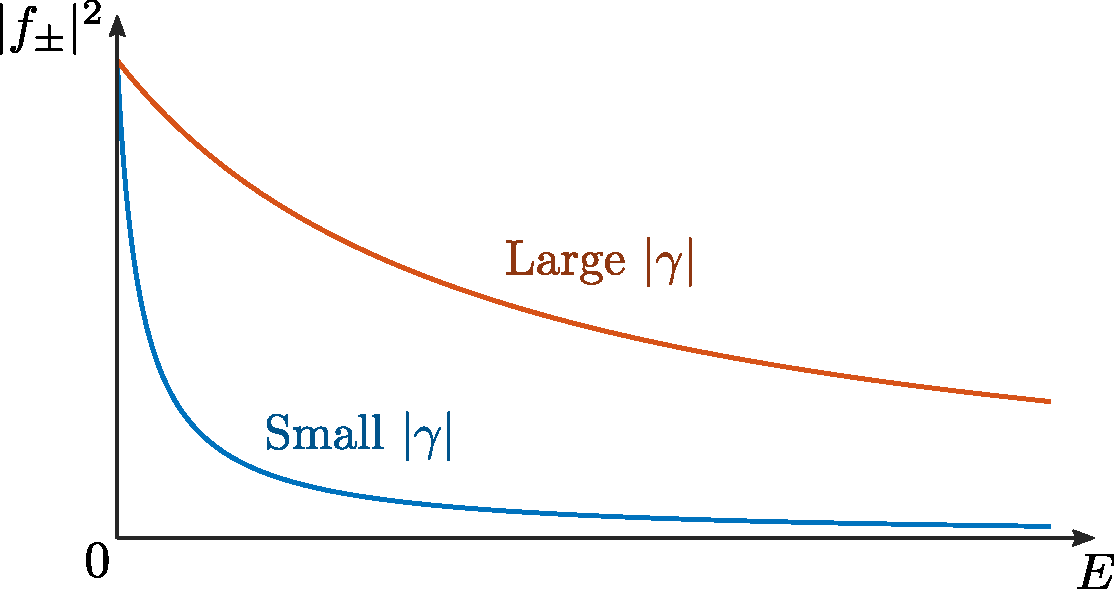
\includegraphics[width=0.5\textwidth]{scattering1df}
\end{figure}

\noindent
The behavior matches our intuition.  For a given particle energy $E$,
the scattering grows stronger as the potential strength parameter
$|\gamma|$ increases.  On the other hand, for fixed $\gamma$, a
higher-energy particle undergoes less scattering.  Note also that
attractive potentials ($\gamma < 0$) and repulsive potentials ($\gamma
> 0$) are equally effective at scattering.

\section{Scattering amplitude and scattering cross section}
\label{sec:scattering_amplitude}

In the 1D scattering problem of the previous section, the particle can
only scatter in two directions: forward or backward.  In 2D and higher
spatial dimensions, there is an important complication: the particle
can also go ``sideways'', and in fact there is a continuous set of
directions for it to scatter into.  To deal with this, physicists have
developed a systematic formalism for expressing the outcomes of
scattering experiments using direction-dependent ``scattering
amplitudes'', which we will now describe.

To begin, let us define the incident wavefunction as a plane wave in
$d$ dimensions, by analogy with the 1D case [Eq.~\eqref{psiin1d}]:
\begin{equation}
  \psi_i(\mathbf{r}) = \Psi_i \, e^{i\mathbf{k}_i\cdot\mathbf{r}},
  \;\;\; |\mathbf{k}_i| = k = \sqrt{\frac{2mE}{\hbar^2}},
  \label{psiin}
\end{equation}
where $\mathbf{k}_i$ is the incident wave-vector and $\Psi_i \in
\mathbb{C}$ is the incident amplitude.

The incident wavefunction generates a scattered wavefunction
$\psi_s(\mathbf{r})$.  We can express the $\mathbf{r}$-dependence of
this wavefunction using a coordinate system of the form $(r,\Omega)$,
where $r$ is the distance from the origin and $\Omega$ denotes the
other ``directional'' coordinates.  Specifically,
\begin{itemize}
\item For $d = 2$, we use polar coordinates $(r,\phi)$, i.e.~$\Omega
  \equiv \phi$.

\item For $d = 3$, we use spherical coordinates $(r, \theta, \phi)$,
  i.e.~$\Omega \equiv (\theta,\phi)$.
\end{itemize}
We can also wrangle the $d = 1$ case into this framework by letting
$\Omega \in \{+, -\}$, where $+$ denotes the forward ($+x$) direction
and $-$ denotes the backward ($-x$) direction.

In a typical scattering experiment, the scattered wavefunction is
detected at $r \rightarrow \infty$; i.e., at distances much longer
than the size of the scatterer, the free-space wavelength, and any
other relevant length scales.  In this regime, we assert that the
scattered wavefunction must reduce to the form
\begin{equation}
  \psi_s(\mathbf{r})\;  \overset{r\rightarrow\infty}{\longrightarrow}\; \Psi_i \, r^{\frac{1-d}{2}} \, e^{ikr} \, f(\Omega).
  \label{psiscat}
\end{equation}
To understand the reasoning behind this, let us go through the
individual multiplicative factors on the right side of
Eq.~\eqref{psiscat}.

The first factor $\Psi_i$ accounts for the fact that the Schr\"odinger
wave equation is linear.  If we vary the incident amplitude, the
scattered wavefunction must vary proportionally.

The next two factors, $r^{\frac{1-d}{2}} \, e^{ikr}$, give the
$r$-dependence of a wave expanding radially from the origin in $d$
dimensions.  The $e^{ikr}$ factor captures its outgoing nature (the
wavefunction's phase increases along the direction of propagation,
i.e., the direction of increasing $r$).  The other factor provides the
$r$-scaling needed for probability conservation.  Note that the
probability current density associated with the scattered wavefunction
is
\begin{equation}
  \mathbf{J}_s = \frac{\hbar}{m} \mathrm{Im}\big[\psi_s^*\nabla\psi_s\big].
\end{equation}
Thus, its radial component is
\begin{equation}
  \begin{aligned}J_{s}^r\; &= \frac{\hbar}{m}\, \mathrm{Im}\left[\psi_s^* \frac{\partial}{\partial r}\psi_s\right] \\
    &\overset{r\rightarrow\infty}{\longrightarrow}\;\, \big(\cdots\big)
    \mathrm{Im}\left[\left(r^{\frac{1-d}{2}} \, e^{ikr}\right)^* \frac{\partial}{\partial r} \left(r^{\frac{1-d}{2}} \, e^{ikr}\right)\right] \\
    &= \big(\cdots\big)\,
    \mathrm{Im}\left[\left(r^{\frac{1-d}{2}} \, e^{ikr}\right)^* \left(ik r^{\frac{1-d}{2}} \, e^{ikr} + \frac{1-d}{2} \, r^{\frac{-1-d}{2}} \, e^{ikr}\right)\right] \\
    &= \big(\cdots\big) \, r^{-(d-1)} + O(r^{-d}),
  \end{aligned}
  \label{Jsrcalc}
\end{equation}
where $(\cdots)$ denotes $r$-independent terms.  In $d$ dimensions,
the area of the surface at distance $r$ from the origin scales as
$r^{d-1}$.  Hence, $J_{s}^r$ scales inversely with area, and the total
flux obtained by integrating $J_{s}^r$ over the area is independent of
$r$.

The final factor in Eq.~\eqref{psiscat}, $f(\Omega)$, is called the
\textbf{scattering amplitude}.  This complex function is typically the
main avenue by which a scattering experiment reveals information about
the scatterer.  As noted in the previous paragraphs, in the large-$r$
limit, the other factors are determined by linearity, outgoing-ness,
and flux conservation.  Hence, only $f$ is sensitive to the details of
the scattering potential.

Note that the scattering amplitude is a function of $\Omega$, i.e.,
the direction of $\mathbf{r}$.  Sometimes, it is written using the
alternative notation
\begin{equation}
  f(\mathbf{k}_i \rightarrow \mathbf{k}_f), \qquad
  \mathbf{k}_f = k\, \frac{\mathbf{r}}{|\mathbf{r}|}.
\end{equation}
This emphasizes that the particle is initially incident with
wave-vector $\mathbf{k}_i$, then gets scattered elastically into a
wave-vector $\mathbf{k}_f$ pointing in the direction of $\mathbf{r}$.

From the scattering amplitude, we can define two other important
quantities:
\begin{framed}
  \begin{align}
    \frac{d\sigma}{d\Omega} &= \big|f(\Omega)\big|^2 \qquad\quad\quad \text{(the \textbf{differential scattering cross section})} \\ \sigma &= \int d\Omega\; \big|f(\Omega)\big|^2 \quad\; \text{(the \textbf{total scattering cross section}).} \label{sigma}
  \end{align}
\end{framed}
\vskip -0.1in
\noindent
In Eq.~\eqref{sigma}, $\int d\Omega$ denotes the integral(s) over all
the angle coordinates.  For 1D, this is replaced by a discrete sum
over the forward and backward directions (see above).

The term ``cross section'' comes from an analogy with the scattering
of classical particles.  Imagine a stream of classical particles
incident on a ``hard-body'' scatterer:

\begin{figure}[h]
  \centering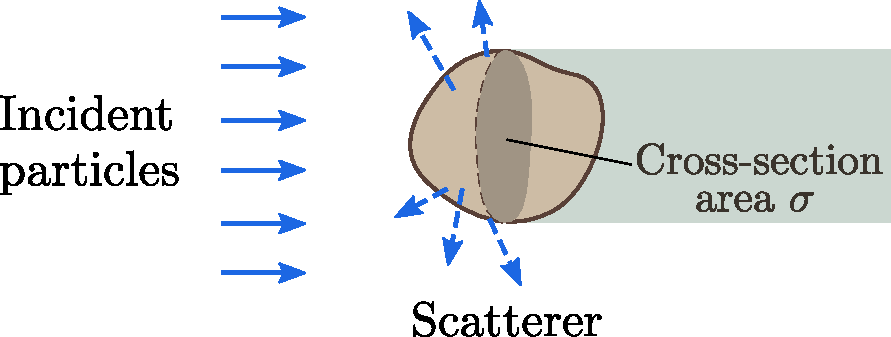
\includegraphics[width=0.44\textwidth]{crosssection}
\end{figure}

\noindent
Let the incident classical particles have the same flux as the
incident wavefunction \eqref{psiin},
\begin{equation}
  J_{i} = \frac{\hbar k}{m} \;|\Psi_i|^2.
  \label{incidentflux}
\end{equation}
Note that this has units of $[x^{1-d}t^{-1}]$ (i.e., number per unit
time per unit area in $d$ dimensions).  We assume the scatterer only
interacts with the particles striking it directly, and the rate at
which these strikes occur is
\begin{equation}
  I_s = J_i \, \sigma,
  \label{scattersigma}
\end{equation}
where $\sigma$ is the exposed cross-sectional area of the scatterer,
as shown in the figure.  This is the \textit{total} rate at which
scattering occurs, regardless of where the particles scatter to.

Let us compare this to the quantum mechanical scattering rate.  Using
Eq.~\eqref{psiscat}, we can repeat the calculation in \eqref{Jsrcalc}
for the radial component of the probability current density:
\begin{equation}
  J_s^r \; \overset{r\rightarrow\infty}{\longrightarrow}\;
  \frac{\hbar \,k}{m}\; |\Psi_i|^2 \; |f(\Omega)|^2 \,r^{1-d}
  + O(r^{-d}).
\end{equation}
Hence, the total flux of outgoing probability is
\begin{equation}
  I_s = \int d\Omega\; r^{d-1} \, J_{s,r}
  = \left(\frac{\hbar k}{m} \;|\Psi_i|^2\right) \; \int d\Omega\; \big|f(\Omega)\big|^2.
  \label{scatterI}
\end{equation}
On the right side, the quantity in parentheses is the incident flux,
Eq.~\eqref{incidentflux}.  Comparing Eq.~\eqref{scatterI} to
Eq.~\eqref{scattersigma}, we see that
\begin{equation*}
  \sigma \equiv \int d\Omega \; \big|f(\Omega)\big|^2
\end{equation*}
is the quantity analogous to the exposed cross-sectional area of the
classical hard-body.  We therefore call this the \textbf{total
  scattering cross section}.

Moreover, the integrand $|f|^2$ represents the rate, per unit of solid
angle, at which particles are scattered in a given direction.  We call
this the \textbf{differential scattering cross section}.  The total
and differential scattering cross sections are the principal
observable quantities typically obtained in scattering experiments.

\section{The Green's function}
\label{sec:greensfun}

The scattering amplitude $f(\Omega)$ can be calculated using a variety
of analytical and numerical methods.  We will discuss one particularly
important approach, based on a quantum variant of the Green's function
technique for solving inhomogenous differential equations.

Let us return to the previously-discussed formulation of the
scattering problem:
\begin{align}
  \begin{aligned} \hat{H} &= \hat{H}_0+\hat{V} \\ \hat{H} |\psi\rangle &= E |\psi\rangle \\ |\psi\rangle &= |\psi_i\rangle \,+\, |\psi_s\rangle \\ \hat{H}_0 |\psi_i\rangle &= E |\psi_i\rangle.\end{aligned}
\end{align}
These equations can be combined as follows:
\begin{align}
  \left(\hat{H}_0 + \hat{V}\right) |\psi_i\rangle + \hat{H} |\psi_s\rangle &= E \left( |\psi_i\rangle + |\psi_s\rangle \right) \\
  \Rightarrow \quad \hat{V} |\psi_i\rangle + \hat{H} |\psi_s\rangle &= E |\psi_s\rangle  \\
  \Rightarrow \quad\; \left(E - \hat{H}\right) |\psi_s\rangle & = \hat{V} |\psi_i\rangle \label{EmHeq}
\end{align}
To proceed, we define an operator called the \textbf{Green's
  function}, which is the inverse of the operator on the left side of
Eq.~\eqref{EmHeq}:
\begin{equation}
  \hat{G}(E) = \big(E-\hat{H}\big)^{-1}.
  \label{Gdef}
\end{equation}
Note that $\hat{G}(E)$ depends parametrically on $E$.  We can now
convert Eq.~\eqref{EmHeq} into
\begin{equation}
  |\psi_s\rangle = \hat{G} \hat{V} |\psi_i\rangle.
  \label{scatterform}
\end{equation}

It will also be useful to define the Green's function for a free
particle,
\begin{equation}
  \hat{G}_0(E)=\big(E-\hat{H}_0\big)^{-1}.
  \label{G0unregulated}
\end{equation}
As we shall see, $\hat{G}_0$ often can be calculated exactly, whereas
$\hat{G}$ typically has no closed-form analytic expression.  Moreover,
we can relate $G$ and $G_0$ as follows:
\begin{align}
  \begin{aligned}
    \hat{G}(E-\hat{H}_0 - \hat{V})\;\; &= I \;\;\;\mathrm{and}\;\; (E-\hat{H}_0 - \hat{V})\hat{G} = I \\ \Leftrightarrow \quad\qquad \hat{G} \hat{G}_0^{-1} - \hat{G}\hat{V} &= I \;\;\; \mathrm{and}\;\;\;\;\, \hat{G}_0^{-1} \hat{G} - \hat{V}\hat{G} \;\;\;= I.
  \end{aligned}
\end{align}
Upon respectively right-multiplying and left-multiplying these equations
by $\hat{G}_0$, we arrive at the following pair of equations, called
\textbf{Dyson's equations}:
\begin{framed}
  \begin{align}
    \hat{G} \;&= \; \hat{G}_0 + \hat{G}\hat{V}\hat{G}_0 \\
    \hat{G} \;&=\; \hat{G}_0 + \hat{G}_0\hat{V}\hat{G} \label{dyson2}
  \end{align}
\end{framed}
\vskip-0.1in
\noindent
These equations are ``implicit'', as the unknown $\hat{G}$ appears on
both the left and right sides.

Applying the second Dyson equation, Eq.~\eqref{dyson2}, to the
scattering problem \eqref{scatterform} gives
\begin{align}
  |\psi_s\rangle
  &= \left(\hat{G}_0 + \hat{G}_0\hat{V}\hat{G}\right) \hat{V}
  \, |\psi_i\rangle \\
  &= \hat{G}_0 \hat{V} \left(\hat{I} + \hat{G} \hat{V}\right) |\psi_i\rangle.
  \label{psis_useful}
\end{align}
Using Eq.~\eqref{scatterform} again, we get
\begin{equation}
  |\psi_s\rangle = \hat{G}_0\hat{V} |\psi\rangle.
  \label{psis_implicity}
\end{equation}
This remains an implicit equation, but the unknown is $|\psi\rangle$
rather than $\hat{G}$.  Note that the results up to this point have
been approximation-free.

One approach to solving Eq.~\eqref{psis_implicity} is to repeatedly
plug its right side back into itself:
\begin{align}
  \begin{aligned}
    |\psi_s\rangle &= \hat{G}_0 \hat{V} \left(|\psi_i\rangle + \hat{G}_0 \hat{V}|\psi\rangle\right) \\
    &= \quad \vdots \\
    &= \left[\hat{G}_0 \hat{V} + (\hat{G}_0 \hat{V})^2 + (\hat{G}_0 \hat{V})^3 + \cdots\right]|\psi_i\rangle.
  \end{aligned}
\end{align}
Or, equivalently,
\begin{equation}
  |\psi\rangle
  = \left[\hat{I} + \hat{G}_0 \hat{V} + (\hat{G}_0 \hat{V})^2 + (\hat{G}_0 \hat{V})^3 + \cdots\right]|\psi_i\rangle.
  \label{bornseries}
\end{equation}
This infinite series is called the \textbf{Born series}.

To interpret this result, let us go to the position basis:
\begin{align}
  \begin{aligned}\psi(\mathbf{r}) = \psi_i(\mathbf{r}) &+ \int d^dr' \langle \mathbf{r} | \hat{G}_0 |\mathbf{r}'\rangle\, V(\mathbf{r}') \psi_i(\mathbf{r}') \\ &+ \int d^dr' d^dr'' \langle \mathbf{r} | \hat{G}_0 |\mathbf{r}'\rangle\, V(\mathbf{r}') \, \langle \mathbf{r}' | \hat{G}_0 |\mathbf{r}''\rangle \, V(\mathbf{r}'') \psi_i(\mathbf{r}'') \;\; + \;\;\cdots\end{aligned}
    \label{Bornposition}
\end{align}
This can be regarded as a description of \textbf{multiple scattering}.
The wavefunction is a superposition of terms involving zero, one, two,
or more scattering events, as shown below:

\begin{figure}[h!]
  \centering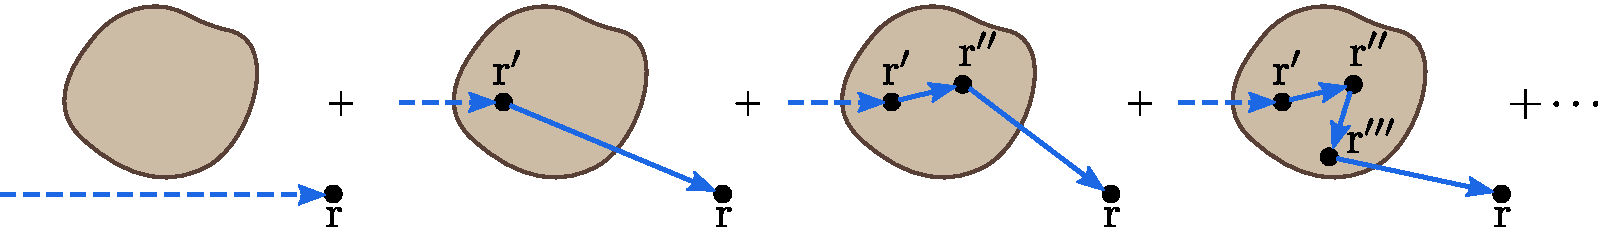
\includegraphics[width=0.9\textwidth]{bornseries}
\end{figure}

\noindent
Each successive term in the Born series involves more scattering
events, i.e., higher multiples of $\hat{V}$.  For example, the
second-order term is
\begin{equation*}
  \int d^dr' d^dr'' \langle \mathbf{r} | \hat{G}_0 |\mathbf{r}'\rangle\, V(\mathbf{r}') \, \langle \mathbf{r}' | \hat{G}_0 |\mathbf{r}''\rangle \, V(\mathbf{r}'') \psi_i(\mathbf{r}''),
\end{equation*}
which describes the particle undergoing (i) scattering of the incident
particle at point $\mathbf{r}''$, (ii) propagation from $\mathbf{r}''$
to $\mathbf{r}'$, (iii) scattering again at point $\mathbf{r}'$, and
(iv) propagation from $\mathbf{r}'$ to $\mathbf{r}$.  Note that
$\mathbf{r}'$ and $\mathbf{r}''$ are integrated over all possible
positions.  Since the integrals are weighted by $V$, the positions
with the strongest scattering potential contribute the most.

For a sufficiently weak scatterer, it is often a good approximation to
retain just the first few terms in the Born series.  The question of
when $\hat{V}$ is ``sufficiently weak''---i.e., when the Born series
converges---is a complex topic beyond the scope of our present
discussion.

\section{Green's function for a free particle}
\label{sec:freegreen}

In the position basis representation of the Born series,
Eq.~\eqref{Bornposition}, a crucial role is played by the matrix
elements $\langle\mathbf{r}|\hat{G}_0|\mathbf{r}'\rangle$.  We call
this the \textbf{propagator}, as it describes how the particle
propagates between discrete scattering events.

Starting from the definition of $\hat{G}_0$ in
Eq.~\eqref{G0unregulated}, we can evaluate it in the position basis:
\begin{align*}
  \langle\mathbf{r} |\big(E-\hat{H}_0\big) \hat{G}_0 |\mathbf{r}'\rangle &= \langle\mathbf{r}|\hat{I}|\mathbf{r}'\rangle \\
  = \left(E + \frac{\hbar^2}{2m}\nabla^2 \right) \langle\mathbf{r} |\hat{G}_0 |\mathbf{r}'\rangle &= \delta^d(\mathbf{r}-\mathbf{r}')
\end{align*}
Hence,
\begin{equation}
  \left(\nabla^2 + k^2\right) \langle\mathbf{r} |\hat{G}_0 |\mathbf{r}'\rangle = \frac{2m}{\hbar^2} \delta^d(\mathbf{r}-\mathbf{r}'),
  \label{propagatoreq}
\end{equation}
where
\begin{equation}
  k^2 = \frac{2mE}{\hbar^2}.
  \label{keq}
\end{equation}
The left side of this equation is the same as the $d$-dimensional
Helmholtz equation, with the $\nabla^2$ acting on the $\mathbf{r}$
coordinates (not $\mathbf{r}'$).  On the right side, we have a term
proportional to a $d$-dimensional delta function at $\mathbf{r} =
\mathbf{r}'$.  The propagator thus describes a wave at each position
$\mathbf{r}$, emitted from a point source at $\mathbf{r}'$.

Eq.~\eqref{propagatoreq} can be solved analytically for different
values of the spatial dimension $d$.  In the following, we will work
through the derivation for $d = 3$.  The derivations for $d = 1$ and
$d = 2$ are left as \hyperref[ex:1dpropagator]{exercises}.

To derive the 3D propagator, we first re-express it using the momentum
eigenbasis:
\begin{align}
  \langle\mathbf{r}|\hat{G}_0|\mathbf{r}'\rangle
  &= \langle\mathbf{r}|\hat{G}_0 \Big(\int d^3k'\; |\mathbf{k}'\rangle\langle\mathbf{k}'| \Big) |\mathbf{r}'\rangle \nonumber \\
  &= \int d^3k' \; \langle\mathbf{r}|\mathbf{k}'\rangle \;
  \frac{1}{E-\frac{\hbar^2|\mathbf{k}'|^2}{2m}} \;
  \langle\mathbf{k}'|\mathbf{r}'\rangle \nonumber \\
  &= \frac{2m}{\hbar^2} \frac{1}{(2\pi)^3} \int d^3k' \;
  \frac{\exp\left[i\mathbf{k}' \cdot
      (\mathbf{r}-\mathbf{r}')\right]}{k^2-|\mathbf{k}'|^2}.
  \label{rGr}
\end{align}
Next, we express $\mathbf{k}'$ using spherical coordinates
$(k',\theta,\phi)$.  We are free to choose the $\theta=0$ axis so that
it points in the direction of $\mathbf{r}-\mathbf{r}'$, as illustrated
below:

\begin{figure}[h]
  \centering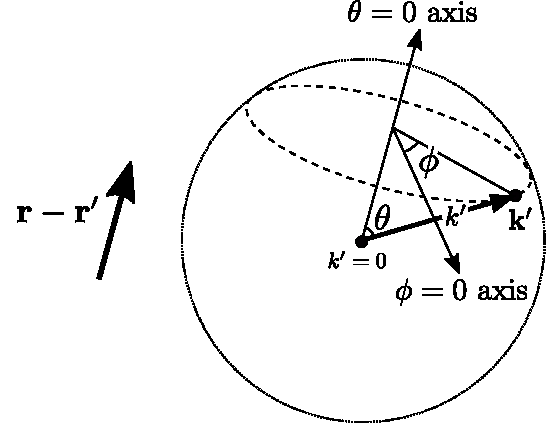
\includegraphics[width=0.4\textwidth]{spherical_coords}
\end{figure}

\noindent
Then,
\begin{align}
  \langle\mathbf{r}|\hat{G}_0|\mathbf{r}'\rangle &= \frac{2m}{\hbar^2} \frac{1}{(2\pi)^3} \int d^3k' \; \frac{\exp\left[i\mathbf{k}'\cdot (\mathbf{r}-\mathbf{r}')\right]}{k^2-|\mathbf{k}'|^2} \nonumber \\
  &= \frac{2m}{\hbar^2} \frac{1}{(2\pi)^3} \int_0^\infty dk' \int_0^\pi d\theta \int_{0}^{2\pi} d\phi \;{k'}^{2}\sin\theta\; \frac{\displaystyle \exp\left(ik'|\mathbf{r}-\mathbf{r}'|\cos\theta\right)}{k^2-{k'}^2} \nonumber \\
  &= \frac{2m}{\hbar^2} \frac{1}{(2\pi)^2} \int_0^\infty dk' \int_{-1}^1 d\mu \;{k'}^2\; \frac{\displaystyle \exp\left(ik'|\mathbf{r}-\mathbf{r}'|\mu\right)}{k^2-{k'}^2} \qquad(\text{letting}\;\mu = \cos\theta) \nonumber \\
  &= \frac{2m}{\hbar^2} \frac{1}{(2\pi)^2} \int_0^\infty dk' \; \frac{ {k'}^2}{k^2-{k'}^2}\, \frac{\displaystyle \exp\left(ik'|\mathbf{r}-\mathbf{r}'|\right) - \exp\left(-ik'|\mathbf{r}-\mathbf{r}'|\right)}{ik'|\mathbf{r}-\mathbf{r}'|} \nonumber\\
  &= \frac{2m}{\hbar^2} \frac{1}{(2\pi)^2} \frac{i}{|\mathbf{r}-\mathbf{r}'|} \int_{-\infty}^\infty dk' \; \frac{\displaystyle k'\, \exp\left(ik'|\mathbf{r}-\mathbf{r}'|\right)}{(k' - k)(k'+k)}.
  \label{rGrintegrand}
\end{align}
This looks like something we can handle via contour integration.  But
there's a snag: the integration contour runs over the real $k'$ line,
but since $k \in \mathbb{R}^+$ the poles at $\pm k$ lie on the
contour.  The integral, as currently defined, is singular.

To get a finite result, we must ``regularize'' the integral by
adjusting its definition.  One way is to perturb the integrand and
shift its poles infinitesimally in the complex plane, moving them off
the contour.  We have a choice of whether to move each pole
infinitesimally up or down.  It turns out that the appropriate choice
is to shift the pole at $-k$ down, and shift the pole at $+k$ up, as
illustrated by the red dots in the following figure:

\begin{figure}[h!]
  \centering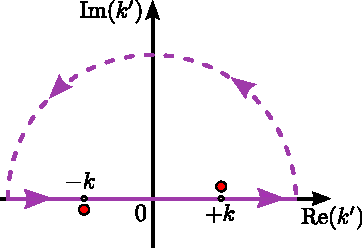
\includegraphics[width=0.34\textwidth]{greencontour}
\end{figure}

\noindent
This alters the denominator in the integrand of
Eq.~\eqref{rGrintegrand} as follows:
\begin{equation}
  (k' - k)(k'+k) \;\rightarrow\; (k' - k - i\epsilon)(k'+k+i\epsilon) = {k'}^2 - (k+i\epsilon)^2,
  \label{kregularization}
\end{equation}
where $\epsilon$ is a positive infinitesimal.  The implications of
this adjustment will be discussed further below.  For now, let us
proceed to do the integral, which is no longer divergent:
\begin{align*}
  \begin{aligned}\int_{-\infty}^\infty dk' \; \frac{\displaystyle k' \exp\left(ik'|\mathbf{r}-\mathbf{r}'|\right)}{(k' - k)(k'+k)} &\rightarrow \lim_{\varepsilon \rightarrow 0^+} \int_{-\infty}^\infty dk' \; \frac{\displaystyle k' \exp\left(ik'|\mathbf{r}-\mathbf{r}'|\right)}{(k' - k - i\varepsilon)(k'+k+i\varepsilon)}\;\;\; (\text{regularize}) \\ &= \lim_{\varepsilon \rightarrow 0^+} \int_C dk' \; \frac{\displaystyle k' \exp\left(ik'|\mathbf{r}-\mathbf{r}'|\right)}{(k' - k - i\varepsilon)(k'+k+i\varepsilon)} \quad\;\;\; (\text{close contour above}) \\ &= 2\pi i \lim_{\varepsilon \rightarrow 0^+} \mathrm{Res}\left[\frac{\displaystyle k' \exp\left(ik'|\mathbf{r}-\mathbf{r}'|\right)}{(k' - k - i\varepsilon)(k'+k+i\varepsilon)}, \;k'=k+i\varepsilon^+\right] \\ &= \pi i \exp\left(ik|\mathbf{r}-\mathbf{r}'|\right).\end{aligned}
\end{align*}
Finally, plugging this into Eq.~\eqref{rGrintegrand} gives the result
\begin{equation}
  \langle\mathbf{r}|\hat{G}_0|\mathbf{r}'\rangle = -\frac{2m}{\hbar^2}
  \cdot \frac{\exp\left(ik|\mathbf{r}-\mathbf{r}'|\right)}{4\pi|\mathbf{r}-\mathbf{r}'|}.
  \label{3dprop}
\end{equation}

The 3D propagator \eqref{3dprop} describes a spherical wave centered
at the source $\mathbf{r}'$.  The wave is isotropic (i.e., independent
of the direction of $\mathbf{r} - \mathbf{r}'$), consistent with the
fact that the source, a delta function, has no preferred direction.
The amplitude of the wave decreases inversely with $\Delta r =
|\mathbf{r}-\mathbf{r}'|$, consistent with flux conservation in 3D
(see Sec.~\ref{sec:scattering_amplitude}).

Most importantly, the wave propagates \textit{outward} from
$\mathbf{r}'$ (since the phase of the wavefunction increases with
$\Delta r$).  Such a propagator is said to be \textbf{causal}, a word
based on the term ``cause and effect''---the wave travels from the
source at $\mathbf{r}'$ (the \textit{cause}) to $\mathbf{r}$ (the
\textit{effect}).  We can trace this behavior back to the
regularization in Eq.~\eqref{kregularization}; other regularization
choices can be shown to yield propagators with different properties
(see \hyperref[ex:anticausal]{exercises}).  Our regularization
\eqref{kregularization} can also be expressed as an infinitesimal
shift in $E$, via Eq.~\eqref{keq}:
\begin{equation}
  \frac{\hbar^2 k^2}{2m} = E
  \;\;\;\Rightarrow\;\;\;
  \frac{\hbar^2 (k+i\epsilon)^2}{2m}
  = \frac{\hbar^2}{2m} \left(k^2 + 2ik\epsilon + \cdots\right)
  = E + i\varepsilon.
\end{equation}
In other words, we have swapped the original definition of the Green's
function, Eq.~\eqref{G0unregulated}, for a \textbf{causal Green's
  function}
\begin{framed}
  \begin{equation}
    \hat{G_0} = \lim_{\varepsilon\rightarrow 0^+} \big(E - \hat{H}_0 + i \varepsilon\big)^{-1}.
    \label{G0regulated}
  \end{equation}
\end{framed}

%% At large distances, the
%% outgoing waves in \eqref{propagator_solutions} go as $\exp(ikr)$, so
%% the correction to $k$ suppresses the wavefunction and makes it
%% integrable.)

Based on Eq.~\eqref{G0regulated}, causal propagators can also be
derived for other dimensions (see
\hyperref[ex:1dpropagator]{exercises}).  The results for $d = 1, 2,$
and $3$ are summarized below:
\begin{framed}
  \begin{equation}
    \langle\mathbf{r}|\hat{G}_0|\mathbf{r}'\rangle = \frac{2m}{\hbar^2} \times \begin{cases} \Bigg.\displaystyle\frac{1}{2ik} \exp\left(ik|x-x'|\right),& d=1\\ \Bigg. \displaystyle\frac{1}{4i} H^+_0(k|\mathbf{r}-\mathbf{r'}|), & d=2 \\ \displaystyle \Bigg. - \frac{\exp\left(ik|\mathbf{r}-\mathbf{r}'|\right)}{4\pi|\mathbf{r}-\mathbf{r}'|}, & d = 3.  \end{cases}
    \label{propagator_solutions}
  \end{equation}
\end{framed}
\vskip -0.1in
\noindent
For each $d$, the causal propagator describes a wave propagating
outward isotropically from $\mathbf{r}'$.  In 1D, this has the form of
a plane wave on each side. In 2D, it is a circular wave ($H_0^+$
denotes a Hankel function; see Appendix A), and in 3D it is a
spherical wave.


%% Alternative tweaks to the Green's function produce different
%% behaviors.  For instance, we could flip the sign of $\varepsilon$
%% in Eq.~\eqref{G0regulated}.  This gives rise to an
%% \textbf{anti-causal Green's function}, whose solutions are
%% \textit{incoming} waves that arrive from infinity and are absorbed
%% into $\mathbf{r}'$.  In dealing with scattering problems, we
%% generally always use the causal Green's function.

\section{Scattering amplitudes in 3D}
\label{sec:3damp}

We are now in a position to generate explicit solutions for the
scattering problem by combining the results of
Sections~\ref{sec:scattering_amplitude}--\ref{sec:freegreen}.  For
ease of presentation, we will focus on the 3D case; the 1D and 2D
cases are handled in a similar way.

Using Eqs.~\eqref{psiscat} and \eqref{psis_useful}, we can write the
scattered wavefunction as
\begin{equation}
  \psi_s(\mathbf{r})
  = \langle\mathbf{r}|
  \hat{G}_0 \hat{V}
  \underbrace{\big(\hat{I} + \hat{G} \hat{V}\big) |\psi_i\rangle}_{= |\psi\rangle}
   \\
  \;\; \overset{r\rightarrow\infty}{\longrightarrow}\;\;
  \Psi_i \, \frac{e^{ikr}}{r} \, f(\mathbf{k}_i\rightarrow k\hat{\mathbf{r}}).
  \label{psis_expansion}
\end{equation}
We want to use this to find the scattering amplitude $f$, which
encodes the results of the scattering experiment in the large-$r$
limit (see Sec.~\ref{sec:scattering_amplitude}).

Let us work on the expression on the left first.  Using the position
representation,
\begin{align}
  \psi_s(\mathbf{r}) = \int d^3r'\; \langle\mathbf{r}|\hat{G}_0|\mathbf{r}'\rangle\, V(\mathbf{r}')\, \langle \mathbf{r}'| \big(\hat{I} + \hat{G} \hat{V}\big) |\psi_i\rangle.
  \label{psis_positionrep}
\end{align}
From Eq.~\eqref{propagator_solutions}, the causal propagator in 3D is
\begin{equation}
  \langle\mathbf{r}|\hat{G}_0|\mathbf{r}'\rangle =
  - \frac{2m}{\hbar^2}
  \frac{\exp\left(ik|\mathbf{r}-\mathbf{r}'|\right)}{4\pi|\mathbf{r}-\mathbf{r}'|}.
\end{equation}
In the $r\rightarrow\infty$ limit, this can be simplified using the
Taylor expansion
\begin{equation}
  |\mathbf{r} - \mathbf{r}'| = r - \hat{\mathbf{r}} \cdot \mathbf{r}' + \cdots,
\end{equation}
where $\hat{\mathbf{r}}$ is the unit vector pointing parallel to
$\mathbf{r}$.  (This is the same large-$r$ expansion used to derive
the electric dipole moment in classical electromagnetism.)  Hence, to
lowest order,
\begin{equation}
  \langle\mathbf{r}|\hat{G}_0|\mathbf{r}'\rangle \overset{r\rightarrow\infty}{\longrightarrow} - \frac{2m}{\hbar^2}\, \frac{e^{ikr}}{4\pi r}\; \exp\left(-ik \, \hat{\mathbf{r}} \cdot \mathbf{r}'\right).
\end{equation}
Applying this to Eq.~\eqref{psis_positionrep} gives
\begin{align}
  \begin{aligned}\psi_s(\mathbf{r})
    &\overset{r\rightarrow\infty}{\longrightarrow} \, - \frac{2m}{\hbar^2} \, \frac{e^{ikr}}{4\pi r}\; \int d^3r' \exp\left(-ik \, \hat{\mathbf{r}} \cdot \mathbf{r}'\right)\, V(\mathbf{r}')\,
    \langle \mathbf{r}'| \big(\hat{I} + \hat{G} \hat{V}\big) |\psi_i\rangle \\
    &\;\;=\;\; - \frac{2m}{\hbar^2} \, \frac{e^{ikr}}{r} \sqrt{\frac{\pi}{2}} \; \big\langle \mathbf{k}_f \big|\hat{V} + \hat{V} \hat{G} \hat{V}
    \big|\psi_i\big\rangle. \end{aligned}
  \label{psis_intermediate}
\end{align}
On the second line, we simplified the expression by introducing the
momentum eigenstate with $\mathbf{k}_f \equiv k \hat{\mathbf{r}}$.
This corresponds to the ``final'' momentum of the scattered particle,
measured when the particle is picked up by a detector placed in the
$\hat{\mathbf{r}}$ direction relative to the origin.  Note that
$|\mathbf{k}_f| = |\mathbf{k}_i| = k$, consistent with elastic
scattering.  Similarly, we can express the incident state in terms of
a momentum eigenstate, by comparing Eqs.~\eqref{kwavefun} to
\eqref{psiin}:
\begin{equation}
  |\psi_i\rangle = \Psi_i (2\pi)^{3/2} |\mathbf{k}_i\rangle.  
\end{equation}
Thus, Eq.~\eqref{psis_intermediate} becomes
\begin{align}
  \begin{aligned}\psi_s(\mathbf{r}) \; &\overset{r\rightarrow\infty}{\longrightarrow} - \frac{2m}{\hbar^2} \, \Psi_i\, \frac{e^{ikr}}{r} \; 2\pi^2 \; \big\langle \mathbf{k}_f \big|\hat{V} + \hat{V}\hat{G}\hat{V}\big|\mathbf{k}_i\big\rangle.\end{aligned}
\end{align}
Comparing this to the right side of Eq.~\eqref{psis_expansion}, we can
read off the scattering amplitude:
\begin{framed}
  \begin{align}
    \begin{aligned}
      f(\mathbf{k}_i \rightarrow \mathbf{k}_f) &= - \frac{2m}{\hbar^2} \,\cdot \, 2\pi^2 \; \big\langle \mathbf{k}_f\big| \hat{V} + \hat{V}\hat{G} \hat{V} \big|\mathbf{k}_i\big\rangle \\
      &= - \frac{2m}{\hbar^2} \,\cdot \, 2\pi^2 \; \big\langle \mathbf{k}_f\big| \hat{V} + \hat{V}\hat{G}_0 \hat{V} + \hat{V} \hat{G}_0 \hat{V} \hat{G}_0\hat{V} + \cdots \big|\mathbf{k}_i\big\rangle.  \end{aligned}
    \label{fresult}
  \end{align}
\end{framed}
\vskip -0.15in
\noindent
As noted above, this result is subject to the elasticity constraint
$|\mathbf{k}_i| = |\mathbf{k}_f|$.  To get the infinite series on the
second line of Eq.~\eqref{fresult}, we have used
Eq.~\eqref{bornseries}.

Eq.~\eqref{fresult} is the culmination of numerous definitions and
derivations from the preceding sections.  On the left side is the
scattering amplitude, the fundamental quantity of interest in a
scattering experiment.  The right side contains the various inputs to
the scattering problem: the initial and final momenta, the scattering
potential, and the Green's function.  Although this result was derived
for the 3D case, very similar formulas hold for other dimensions, with
the $2\pi^2$ factor replaced with other numerical factors.

\section{Example: uniform spherical well in 3D}

Let us test the Born series with a simple scatterer.  Consider a
scattering potential that consists of a uniform spherical well of
depth $U > 0$ and radius $R$:
\begin{equation}
  V(\mathbf{r}) = \begin{cases}-U, & |\mathbf{r}| \le R \\ \;\;\;\,0,
    & |\mathbf{r}| > 0. \end{cases}
\end{equation}

As it turns out, this particular scattering problem can be solved
exactly by exploiting the spherical symmetry of $V(\mathbf{r})$.  The
solution method, called \textbf{partial wave analysis}, is explained
in \textbf{Appendix A}.  Its result is
\begin{equation}
  \begin{aligned}f(\mathbf{k}_i \rightarrow \mathbf{k}_f) &= \frac{1}{2ik}\, \sum_{\ell =0}^\infty \big(e^{2i\delta_\ell} - 1\big) \big(2\ell+1\big)\, P_{\ell}(\hat{\mathbf{k}}_i\cdot \hat{\mathbf{k}}_f), \\ \mathrm{where}\;\; \delta_\ell &= \frac{\pi}{2} + \mathrm{arg}\!\left[k {h_\ell^+}'(kR) \, j_\ell(qR) - qh_\ell^+(kR)\, j_\ell'(qR)\right], \\ q &= \sqrt{2m(E+U)/\hbar^2} \\ k &\equiv |\mathbf{k}_i| = |\mathbf{k}_f|.\end{aligned}
  \label{fresult_well}
\end{equation}
The solution is expressed in terms of the special functions $j_\ell$
(spherical Bessel function of the first kind), $h_\ell^+$ (spherical
Hankel function of the first kind), and $P_\ell$ (Legendre
polynomial).

We will pit this against the Born series, which can be regarded as a
more general method since it does not assume spherical symmetry.
According to Eq.~\eqref{fresult}, the Born series gives
\begin{equation}
  f(\mathbf{k}_i\rightarrow \mathbf{k}_f) = - \frac{2m}{\hbar^2} \,\cdot \, 2\pi^2 \, \left[\big\langle \mathbf{k}_f\big| \hat{V}|\mathbf{k}_i\big\rangle + \big\langle \mathbf{k}_f \big| \hat{V}\hat{G}_0 \hat{V} \big|\mathbf{k}_i\big\rangle + \cdots \right].
  \label{fexpression}
\end{equation}
Evaluating the full infinite Born series is generally an intractable
problem, but we can truncate it to get an approximation for $f$.  For
example, if we keep only the first term, the result is called the
\textbf{first Born approximation}; if we keep only the first two
terms, we obtain the \textbf{second Born approximation}.  To evaluate
the various bra-kets, we can use the position representation to
express them as explicit integrals.  For example,
\begin{align}
  \big\langle \mathbf{k}_f\big| \hat{V}|\mathbf{k}_i\big\rangle
  &= \int d^3r_1\; \frac{\exp(-i\mathbf{k}_f \cdot \mathbf{r}_1)}{(2\pi)^{3/2}} \, V(\mathbf{r}_1) \, \frac{\exp(i\mathbf{k}_i \cdot \mathbf{r}_1)}{(2\pi)^{3/2}}
  \nonumber \\
  &= - \frac{U}{8\pi^3} \int_{|\mathbf{r}_1| \le R} d^3r_1 \; \exp\left[i(\mathbf{k}_i-\mathbf{k}_f)\, \cdot\, \mathbf{r}_1\right] \label{singleint}\\
  \big\langle \mathbf{k}_f \big| \hat{V}\hat{G}_0 \hat{V} \big|\mathbf{k}_i\big\rangle &=
  \int d^3r_1 \!\! \int d^3r_2 \; \frac{\exp(-i\mathbf{k}_f \cdot \mathbf{r}_2)}{(2\pi)^{3/2}} \, V(\mathbf{r}_2) \, \langle\mathbf{r}_2|\hat{G}_0|\mathbf{r}_1 \rangle \, V(\mathbf{r}_1)\, \frac{\exp(i\mathbf{k}_i \cdot \mathbf{r}_1)}{(2\pi)^{3/2}} \nonumber \\
  &= - \frac{U^2}{32\pi^4} \, \frac{2m}{\hbar^2}\, \int_{|\mathbf{r}_1|<R} d^3 r_1 \int_{|\mathbf{r}_2|<R} d^3 r_2 \; \frac{\exp\left[i(k|\mathbf{r}_1-\mathbf{r}_2| - \mathbf{k}_f \cdot \mathbf{r}_2 +\mathbf{k}_i \cdot \mathbf{r}_1)\right]}{|\mathbf{r}_1-\mathbf{r}_2|}.
  \label{doubleint}
\end{align}

To evaluate the integrals, an expedient approach is
\href{https://en.wikipedia.org/wiki/Monte_Carlo_integration}{Monte
  Carlo integration}.  For instance, the integral \eqref{singleint}
has the form
\begin{equation}
  I = \int_{|\mathrm{r}|<R} d^3r \, F(\mathbf{r}).
\end{equation}
To compute this, we randomly sample $N$ points within a cube of volume
$(2R)^3$ centered at the origin.  Note that this cube encloses the
radius-$R$ sphere over which is the integration region.  For each
sampled point, $\mathbf{r}^{(n)}$, we take
\begin{equation}
  F_n = \begin{cases}F(\mathbf{r}^{(n)}), & |\mathbf{r}^{(n)}| < R \\ 0, &\mathrm{otherwise},\end{cases}
\end{equation}
which drops contributions from points outside the sphere.  Then our
estimate for $I$ is
\begin{equation}
  I \,\approx\, (2R)^3 \, \langle F_n\rangle \,=\, \frac{(2R)^3}{N} \sum_{n=1}^N F_n.
  \label{Iest}
\end{equation}
The estimate converges to the true value as $N\rightarrow\infty$.  In
practice, $N \sim 10^4$ yields a good result for typical 3D integrals,
and can be calculated in seconds on a modern computer.

Similarly, to calculate a double integral like Eq.~\eqref{doubleint},
we sample \textit{pairs} of points, $(\mathbf{r}_1^{(n)},
\mathbf{r}_2^{(n)})$, and replace the volume factor $(2R)^3$ in
Eq.~\eqref{Iest} with $(2R)^6$.  The rest of the estimation procedure
is the same.

In the figure below, we compare the Born approximation to the exact
solution \eqref{fresult_well}.  We plot $|f|^2$ versus the energy $E$
at a $90^\circ$ scattering angle (i.e., $\mathbf{k}_f$ perpendicular
to $\mathbf{k}_i$), for fixed well radius $R = 1$ and two well depths,
$U = 0.1$ and $U = 1$.  We adopt computational units $\hbar = m = 1$,
and compute each Monte Carlo integral using $3\times10^4$ samples.

\begin{figure}[h]
  \centering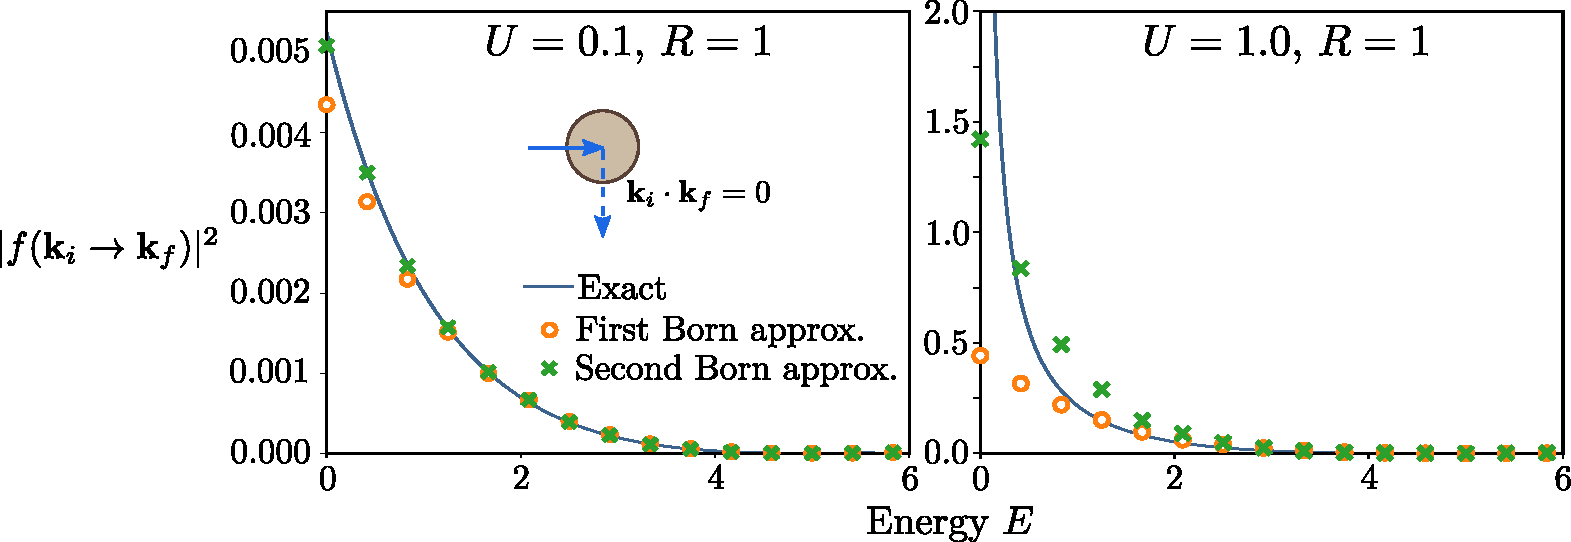
\includegraphics[width=0.97\textwidth]{spherical_well_scattering}
\end{figure}

The first thing to notice is that $|f|^2$ diminishes to zero for large
$E$.  This makes sense: the scattering potential has some energy scale
$\sim U$, so a particle with energy $E \gg U$ should simply zoom
through, with little chance of being deflected.

Looking more closely, we see that for the shallower well ($U = 0.1$),
the first Born approximation already agrees quite well with the exact
results.  However, the second Born approximation is significantly more
accurate, particularly for small $E$.

For the deeper well ($U = 1$), neither the first nor second Born
approximations do a good job.  Roughly speaking, for the deep
potential well, we cannot neglect multiple-scattering events
represented by higher terms in the Born series, whereby the particle
bounces around many times before leaving the scatterer (see
Sec.~\ref{sec:greensfun}).

In fact, for very strong scattering potentials, even taking the Born
approximation to high orders may not work, as the Born series may
become non-convergent.  In such cases, different methods must be
brought to bear.  We will see an example in the next chapter.

\section*{Exercises}

\begin{enumerate}
\item In Sec.~\ref{sec:waves}, we derived the eigenstates of a
  particle in an empty infinite space by considering a box of length
  $L$ on each side, applying periodic boundary conditions, and taking
  $L \rightarrow \infty$.  Suppose we instead use Dirichlet boundary
  conditions (i.e., the wavefunction vanishes on the walls of the
  box).  Show that this gives rise to the same set of momentum
  eigenstates in the $L \rightarrow \infty$ limit.

\item Using the results for the 1D delta-function scattering problem
  described in Section~\ref{sec:1dscatter}, calculate the probability
  current
  \begin{equation}
    J(x) = \frac{\hbar}{2mi}\left(\psi^*\frac{d\psi}{dx} - \psi\frac{d\psi^*}{dx}\right),
  \end{equation}
  where $\psi(x)$ is the \textit{total} (incident + scattered)
  wavefunction.  Explain the relationship between the values of $J$ on
  the left and right side of the scatterer.

\item \label{ex:1dpropagator}
  Derive the causal 1D propagator:
  \begin{equation}
    \langle x|\hat{G}_0|x'\rangle = \frac{2m}{\hbar^2} \cdot \frac{1}{2ik_i} \exp\left(ik_i|x-x'|\right).
  \end{equation}

\item \label{ex:2dpropagator}
  Derive the causal 2D propagator:
  \begin{equation}
    \langle\mathbf{r}|\hat{G}_0|\mathbf{r}'\rangle = \frac{2m}{\hbar^2}\;
    \frac{1}{4i} H^+_0(k|\mathbf{r}-\mathbf{r'}|).
  \end{equation}
  You should be able to adapt many of the steps in the 3D propagator
  derivation from Section~\ref{sec:freegreen}.  When evaluating the
  polar integral, you may want to refer to the discussion of Bessel
  and Hankel functions in Appendix A.  You may also need the following
  mathematical identity between the Hankel functions:
  \begin{equation}
    H_m^+(z) = - (-1)^m \, H_m^-(-z).
  \end{equation}
  
\item \label{ex:anticausal}
  In place of the causal Green's function defined in
  Eq.~\eqref{G0regulated}, consider an infinitesimal shift of the
  opposite sign:
  \begin{equation}
    \hat{G_0} = \lim_{\varepsilon\rightarrow 0^+} \big(E - \hat{H}_0 - i \varepsilon\big)^{-1}.
    \label{G0anticausal}
  \end{equation}
  \begin{enumerate}[(a)]
  \item 
  Whereas the causal propagators in Eq.~\eqref{propagator_solutions}
  represent outgoing waves, explain why Eq.~\eqref{G0anticausal} will
  give rise to propagators representing incoming waves.

\item  In the derivation of the 3D propagator,
  Eqs.~\eqref{rGr}--\eqref{3dprop}, show mathematically how
  Eq.~\eqref{G0anticausal} changes the contour integration, resulting
  in an incoming-wave solution.
  \end{enumerate}

\item In Section~\ref{sec:3damp}, the scattering amplitude
  $f(\mathrm{k}\rightarrow\mathrm{k}')$ for the 3D scattering problem
  was derived using the Born series.  Derive the corresponding
  expressions for 1D and 2D.
\end{enumerate}

\section*{Further Reading}

\begin{enumerate}[[1{]}]
\item Bransden \& Joachain, \S13.1---13.3 and \S13.5---13.6.
\item Sakurai, \S7.1--7.3, 7.5--7.6
\end{enumerate}

\end{document}


%% For decades after the discovery of quantum mechanics, the quantum
%% double-slit experiment was just a ``thought experiment'', meant to
%% illustrate the features of quantum mechanics that had been uncovered
%% by other, more complicated experiments.  Nowadays, the most convenient
%% way to do the experiment is with light, using single-photon sources
%% and single-photon detectors.  Quantum interference has also been
%% demonstrated experimentally using electrons, neutrons, and even
%% large-scale particles such as buckyballs.
